\documentclass[conference]{IEEEtran}
\usepackage{fancyhdr}\usepackage[utf8]{inputenc}
\usepackage{graphicx}
\usepackage{multirow}

\usepackage{lastpage}

%\usepackage{draftwatermark}


%\SetWatermarkText{UoA}
%\SetWatermarkScale{3}

\pagestyle{fancy}
\fancyhf{}
\rfoot{Page \thepage \hspace{1pt} of \pageref{LastPage}} 

\title{Is it Possible to Extend IPv6?}
\date{December 2022}

\author{\IEEEauthorblockN{Ana Custura}
\IEEEauthorblockA{
\textit{University of Aberdeen}\\
}
\and
\IEEEauthorblockN{Raffaello Secchi}
\textit{University of Aberdeen}\\
\and
\IEEEauthorblockN{Gorry Fairhurst}
\textit{University of Aberdeen}\\
}
\begin{document}

\maketitle

\begin{abstract}
The IPv6 Hop-by-Hop Options and Destination Options Extension Headers have historically faced challenges in deployment due to the lack of support in hardware-based forwarding and concerns around potential denial-of-service attacks. However, there has been a renewed interest within the standards community both in simplifying their processing, and in using them for new applications. 
Through a wide-scale measurement campaign, we show that many Autonomous Systems (ASes) in access networks and core of the Internet permit the traversal of EHs including Options, and that path traversal is highly variable depending on the type of network, size of option and transport protocol used, but not on the type of option sent. We also show that packets including Extension Headers can impact load balancing network functions, and present evidence of equipment misconfiguration. Finally we outline the remaining deployment challenges for the EHs and provide recommendations for utilizing them.

\end{abstract}

\begin{IEEEkeywords}
IPv6 protocol, Extension Headers, Protocol Evolution
\end{IEEEkeywords}

\section{Introduction}
\label{sec:introduction}

XX 
REFER TO:
Review of Approaches for the use of the Label Flow of IPv6 Header
https://ieeexplore.ieee.org/document/7014534

XX
IPv6 Extension Headers (EHs)~\cite{RFC8200} are optional headers that a source node can
add to the base IPv6 header to include extra functionality and features as a packet traverses an IPv6 network path. They were defined in the IPv6 specification
to ensure the protocol was flexible and extensible.
%The use of extension headers allows for a flexible and extensible design of IPv6 that can support a variety of new networking features and technologies.
% commented out as it does not say much
IPv6 EHs are widely used to implement some specific functions. However, there has been low levels of network support for two key EHs: the Destination header (DST) and the Hop-by-Hop (HBH) header~\cite{rfc9098}. One reason cited for this is that network devices, such as firewalls, routers, load balancers and intrusion detection systems do not properly handle packets including an EH, that can result in a drop of the packet including the EH (i.e., the packet fails traverse the end-to-end network path).
Additionally, some network administrators can implement a firewall policy that discards packets including an EH to mitigate security concerns, such as to bypass
security mechanisms or to launch Denial of Service (DoS) attacks~\cite{naagas2021deh}.

Plausible reasons for limited traversal of packet including EHs are documented~\cite{ietf-v6ops-HBH-03}, where the authors note that early IPv6 routers
processed EHs in software. This processing of EHs would normally utilise the slow-path, rather than the optimised fast-path, resulting in decreased router forwarding rates. In some designs, this processing consumed resources that would normally be used for Control Plane processing, opening-up a potential DoS attack vector on the critical router functions (reducing ability to perform routing, management, etc). This motivated network operators to discard packets that include EHs~\cite{rfc9098}.  This, in turn,
discouraged use of EHs and their successful standardisation. 

However, there have been important recent changes that motivate the need to take a fresh look at the use-ability of EHs as a mechanism to extend IPv6. First, modern high-speed routers have introduced hardware support for forwarding that could include the flexibility to parse and process simple headers within the fast-path~\cite{cisco-silicon-one}; specific use-cases have emerged where there is an operational demand for new techniques that could be met by using EH.

%XXX at some point here we will include a ref to ASIC XXX

The paper tries to understand whether these changes in operations and equipment have impacted the forward of packets that include EHs, and seek to understand the opportunity to use EH to implement new functions. It begins by discussing previous independent measurements that have reported contrasting results on the traversal of IPv6 packets that include an EH ~\cite{RFC7872} \cite{apnic} \cite{nalini-iepg114} \cite{james}. The differences between the results are analysed.

The paper then reports a broad dataset collected to explore key aspects (e.g., the size of the EH, the choice of transport, and composition of the EH options) revealing a more diverse and nuanced picture of Internet paths than was previously reported.

%XXX Unsure I think the next para is well placed, nor necesarily the correct story ... the shape of this depends on journal style XXX

Specifically, this research demonstrates that if the EHs are limited in size,
packets including Destination Options can traverse as many as
95\% of a diverse set of Internet paths.  On the one hand, packets including a Hop-by-Hop Options EH only traverse a narrow set of paths. On the other hand, when we
characterise whether these packets traverse Autonomous Systems (AS), if we exclude operator policies in access and transit networks, we find many ASes allow transparent forwarding of EHs.
This paper also presents novel insights into how the inclusion of EHs in packets
impacts the forwarding from source to destination. Our research findings
demonstrate that the inclusion of EHs in packets on paths with a form of network layer load-balancing often results in a narrower set of forwarding paths. Although one could interpret this as an
alternative approach to extracting entropy from EHs, it is more likely a
pathological outcome of load balancing network devices not properly equipped
to handle packets including EHs.
We claim that eliminating these pathologies would open up opportunities for
developers and network operators to take advantage of a range of recently-standardised or in-progress innovative ideas based on EHs, such as sending larger packets~\cite{rfc9268} or monitoring network
performance~\cite{rfc8250}~\cite{ietf-ippm-ioam-ipv6-options-10}.

%XXX Summary para below XXX

The remainder of this paper is organised as follows:  Section~\ref{sec:background} presents
the required background for IPv6 EHs and describes the historical challenges related to
their deployment.  The previous literature describing measurement of paths using IPv6
EHs is surveyed in Section~\ref{sec:motivation}.
Sections~\ref{sec:methodology}-\ref{sec:pathspider-results} present the
methodology and results of this study, organised by the type of network path.  The
implications of our results are discussed in Section~\ref{sec:discussion}.
Finally, the conclusion summarises our findings.

\section{Extending IPv6}
\label{sec:background}

\label{sec:ipv6-option-deployment}

\begin{figure}
\centering
  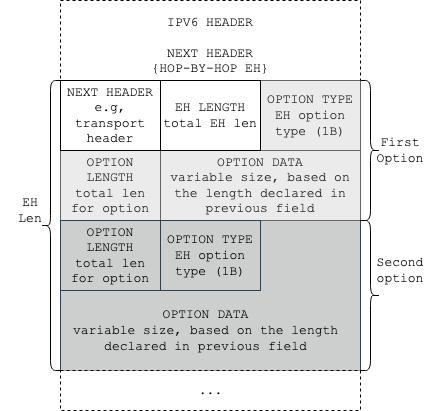
\includegraphics[width=0.5\textwidth]{ehformat.png}
  \caption{IPv6 packet with a base header and two EHs}
  \label{fig:eh-format}
\end{figure}


The original IPv6 specification~\cite{rfc2460} introduced a flexible header structure consisting of a
fixed-length base header and one or more optional Extension Headers (EHs). IPv6 became a full standard in 2017~\cite{RFC8200}. This updated RFC 2460, and also changed some of the processing rules for EHs to align with the current operational practice.

The type of the first EH is denoted in the Next Header field of the IPv6 base header. Each consecutive EH contains a Next Header field to specify the type of the following EH, forming a chain terminated by the IPv6 payload. Each EH also contains a Length field specifying its total length. Figure~\ref{fig:eh-format} shows the structure of an IPv6 packet including a base header followed by a HBH EH containing two Options.

Each EH carries a set of Options. Options uses a Type-Length-Value (TLV) encoding~\cite{RFC8200} with 1~byte for each of the Type and Length fields, and a variable-sized Value field that carries the option data. Although EHs use variable size headers, their total length is always a multiple of 8 bytes to preserve alignment.

The types of EH include: Hop-by-Hop Options (HBH), Routing, Fragment, and
Destination Options (DST). The DST EH is the only EH which is permitted to be included more than once (i.e., it can appear before and after the routing header).

RFC 8200~\cite{RFC8200} allows any sequence of EHs in a single packet providing that they can fit the first fragment in case of fragmentation.

XXX any sequence? - check - I thought defined the sequence XXX 

XXX Below: Not quite - mention  intermediate routers on the path procesing outer DO XXX

A DST EH placed before the payload is meant to be consumed at the final destination endpoint. This is propagated transparently over a network path.

Other EHs could be processed by routers along the path.When the HBH EH is included, it must be placed immediately after the base header~\cite{RFC8200}.

A router can skip any Options that it does not understand. In addition, when an option is unknown, the two most significant bits of the Type
specify the action the device should take to address the unrecognised header. When the two most significant bits are 00, the device should
ignore the option and continue processing the header. If these bits are 01, the
processing should stop and discard the packet. If the bits are 10,
the packet should be discarded and an ICMP notification should be returned to
the sender. Finally, if the bits are 11, the same actions as for 10 should occur,
but this notification should be sent only if the destination address was not multicast. 

Table~\ref{tbl:options} presents the currently standardised 
Options.  We observe that the most Options choose to set the two most significant bits
(MSBs) to 00.  The third most significant bit specifies, if set, that the option data field can be modified en route.

Because HBH Options can be modified by network devices on a path, packets they can be used to provide and collect data from devices on the path to support measurement. This provides an alternative to traditional mechanisms for measurement (e.g., using ICMP):
Option 0x30 provides additional input to inform  PMTUD or PLPMTUD~\cite{rfc9268}, option
0x12 has been specified to measure packet loss, latency, and jitter on live
traffic measurement~\cite{rfc9343} and recently-proposed option 0x31 records
operational and telemetry information that can be updated by devices on the
path between two endpoints. 
Originally, all devices on a path were required to examine and process the HBH EH~\cite{rfc2460}. This requirement was updated by~\cite{RFC8200} to
only apply to devices that have been explicitly configured to process it.


DST can provide similar functionality - Option 0x0F~\cite{rfc8250} can measure performance and diagnostic metrics such as round-trip delay. Other applications can include HBH in packets to improve the reliability of packet forwarding in lossy networks.


% The total EH length is 8-byte aligned and specified in the
% EH Length field, while each individual option declares its own length in the
% Option Length field. 

\begin{table}[b]
\center
\caption{Standardised DSTs and HBHs.}
\begin{tabular}{p{0.03\textwidth}|p{0.055\textwidth}|l|p{0.18\textwidth}}
Hex  & MSBs & Type      & Description                                              \\
\hline
\hline
0x00 & 000  & HBH, Dest & Pad1 (padding)                                           \\
0x01 & 000  & HBH, Dest & PadN (padding)                                           \\
0xC2 & 110  & HBH       & Enable jumbo payloads                                    \\
0x23 & 001  & HBH       & Low-Power and Lossy Networks routing                     \\
0x04 & 000  & Dest      & Mechanism for IPv6 encapsulation                 \\
0x05 & 000  & HBH       & Mechanism for requesting router processing, Router Alert              \\
0xC9 & 110  & Dest      & Mobility Support in IPv6                                 \\
0x8C & 100  & Dest      & Method for identifying subscribers in broadband networks \\
0x6D & 011  & HBH       & Multicast Protocol for Low-Power and  Lossy Networks     \\
0x0F & 000  & Dest      & Delay measurement                                        \\
0x30 & 001  & HBH       & PathMTU                                     \\
0x11 & 000  & HBH, Dest & \multirow{2}{*}{On-path operational info}                \\
0x31 & 001  & HBH, Dest &                                                          \\
0x12 & 000  & HBH, Dest & On-path telemetry                                       
\end{tabular}
  \label{tbl:options}
\end{table}


\subsection{Previous Studies of IPv6 EHs}

\label{sec:motivation}

The debate on whether or not, IPv6 packets that include EHs traverse the Internet is not new to the Internet community.

In 2015, an Informational IETF document presenting traceroute active
measurements to destinations within the Alexa top 1M domains~\cite{RFC7872}
revealed that packets including EHs experience a significantly higher drop rate over an
Internet path compared to packets that do not include EHs. Since then, other
studies~\cite{james}~\cite{nalini-iepg114}~\cite{apnic} have appeared within the standards community that support this claim.  However,
the level and nature of the reported loss varied significantly in these
reports.  This suggests the need for more analysis into the causes of loss and the need to define new measurement methods~\cite{james}~\cite{elkins-v6ops-eh-deepdive-fw-01}.  

XXX This next para seems odd to me... and the CDN case is a little dubious XXX
XXX  this exists and we need to report in it.

A recent IETF draft~\cite{elkins-v6ops-eh-deepdive-fw-01} proposes a new
methodology for isolating the reasons behind EH packet drops and pinpoint the
responsible devices. This focuses on cases where the tested
server is behind a CDN (Content Delivery Network).  While no measurement are included in this document, the authors reported separately on a successful FTP experiment with a DST between 6 vantage points~\cite{nalini-iepg114}.

Another IETF draft, ``Just Another Measurement of Extension header
Survivability" (JAMES)~\cite{james}, presents results on EH path traversal using
traceroute measurements over a mesh network with 21 vantage points located in a set of globally distributed Autonomous Systems (ASes). This study tests all the standardised EHs
(including Routing, Fragment, etc.) in a setting where both ends of the
communication path are under the control of the researcher.  This study found
that only 8-9\% of paths support an 8B HBH, and a 97\% traversal for an 8B
DST. The percentage decreases as the size of the EH
increases~\cite{james-imc}.  We note 6 of the 21 vantage points were
hosted by Digital Ocean\texttrademark, a Cloud provider that does not support
HBH in their networks.

An innovative measurement methodology was built to analyse end-to-end path traversal
rates for Fragmentation, HBH and DST by engineers in APNIC~\cite{apnic}.  This technique initiates TCP connections from clients using a crowd-sourced approach. It performs 
end-to-end measurements by replying to requests with packets that include an EH. If a client then replies to the EH packet, the test is considered successful.  
APNIC reports a volume of 4M measurements/day from clients across most of the IPv6 internet. 
Their findings show that 50\%  of clients reply where DST is used and close to zero where HBH is used.
However, we note that this test does not simply measure traversal over an Internet path, but also whether or not end-user devices reply to a packet that includes an Option. 
%We also note that all measurements were performed from servers in a
%single Cloud provider (Linode).

% The different results outlined above present conflicting views, representative
% of the complex nature of Internet paths. We argue the differences are explained
% by examining the types of networks measured and the choice of vantage points
% and destinations. To fully explore the various aspects of EH traversal, our
% work takes a large-scale measurement approach, testing a wide range of access,
% core and server edge networks, and focuses on the HBH and DST EH types.
% In Section~\ref{sec:discussion}, our results from measurements in access
% networks are compared and discussed alongside their closest counterpart - the
% measurements presented in JAMES~\cite{james}. As we also test edge paths to
% target servers based on top 1M domains lists, we refresh the data presented
% in~\cite{RFC7872} for a longitudinal view.

A large passive measurement campaign used the Czech Republic national
research and education network to analyse IPv6 traffic over a period of one month in
2016~\cite{passive-threats}. It was found that 0.1\% of IPv6 flows
contained an EH, out of which 40.9\% were HBH packets carrying ICMPv6
payloads, primarily multicast (although not specified by the original authors,
we identify this as Multicast for Low-Power and Lossy Networks~\cite{RFC7731}).
The study noted that dropping ICMPv6 traffic that contains EHs could result in
loss of essential network control information. 

% With the exception of~\cite{james-imc}, there are no other peer-reviewed active
% measurement studies. 

Our large-scale measurement study complements the previous analyses. It not only
looks at the end-to-end support in servers, but also provides comparative path
analysis and longitudinal changes in the traversal for HBH and DST.

\subsection{Challenges and Operational Considerations}

XXX next para on architecture XXX

The parsing of IPv6 packets that includes an EH depends on 
the device implementation and
architecture. As the Internet emerged and became widespread, high speed routers have adopted a split architecture, 
with a forwarding plane~\cite{RFC3654} often utilising hardware support, and a control plane, implemented in software (also used for router-critical operations used to manage and control the router)~\cite{router-architecture}.

%In this architecture, incoming packets can be processed on the ``fast path" in the forwarding plane on an Application Specific Integrated Circuits (ASIC) or sent for processing over an internal link on the ``slow path", or the control plane of a router. 

As IPv6 emerged, router architectures have been designed that process all packets that include EHs using the ``slow path"~\cite{ietf-v6ops-hbh-03}.  This resulted in exposing these routers to DoS attacks~\cite{naagas2021deh}, because attacks sending a large amount of IPv6 traffic including EHs could target the router control plane functions where no rate-limiting of such packets was available. This encouraged
network operators to configure their devices to discard packets that included an EHs
in particular the HBH EH~\cite{ietf-v6ops-hbh-03}. We show this filtering likely remains a challenge to EH deployment.

In addition, certain network devices need to inspect the transport protocol information. For example, to inspect ports in the upper-layer protocol header to implement an access control list (ACL) or another security policy.
This requires parsing the entire IPv6 header chain, from the base header to the last EH. 
Such devices are common at a network domain edge, including the edge of enterprise and home networks.

Other examples utilising upper layer protocol headers include: Routers performing Equal Cost Multipath Routing (ECMP), application-layer load balancing, Multi-field classifiers for QoS; deep packet inspection (DPI) and Denial of Service (DoS) attack mitigation. 
XXX
Refer a little to:
Classification of Load Balancing in the Internet - both v4 and v6, interesting note on diamond depth - which might start to answer one of our questions
https://ieeexplore.ieee.org/document/9155387

Some devices might also discard packets including EHs due to buggy implementations.

XXX We can't say this without a good reference

XXX Below is true, but seems like a stub that needs more explanation XXX

A different set of considerations apply to network devices that operate in the Internet core, which typically do not require upper-layer protocol information.
RFC 9288~\cite{rfc9288}  provides recommendations for transit routers. While the document recommends packets on the fast path, or using the slow path providing that there  is a mechanism to control the  packet rate. Where no mitigation options are present, this recommends to discard packets that include these EH. 


%In the early Internet, packet routers were implemented entirely
%in software, and as the Internet grew packet processing was moved from software
%to Application Specific Integrated Circuits (ASICs), while the control
%functions remained~\cite{router-architecture}. Routers started having a split
%architecture with a control and forwarding plane~\cite{RFC3654}, corresponding
%to router-critical operations running in software and hardware processing
%respectively. 
%In this architecture, incoming packets can be processed on the
%``fast path" in the forwarding plane on an ASIC or sent for processing over an
%internal link on the ``slow path", or the control plane of a router. 

%As IPv6 emerged, ASIC support for it was limited, and IPv6 deployment itself was in its infancy - and many network device architectures processed packets containing IPv6 EHs in software~\cite{ietf-v6ops-hbh-03}.  This resulted in opening these routers up to DoS attacks~\cite{naagas2021deh}, because clients sending a large amount of IPv6 traffic including EHs could affect a router's control plane functions where no rate-limiting of such packets was available. This steered
%network operators to configure their devices to discard packets containing EHs,
%in particular the HBH EH~\cite{ietf-v6ops-hbh-03}.

%https://ieeexplore.ieee.org/stamp/stamp.jsp?tp=&arnumber=7949061

%\subsection{Hop-by-Hop and Destination Option EHs}

%An IPv6 packet can contain zero or more EHs, each identified by its own number
%in the Next Header field in the preceding header. The HBH header is
%indicated by the value 0, while the assigned protocol number for the DST
%header is 60. Both HBH and DST can be included in the same IPv6 packet in
%different EHs. An EH can contain multiple Options - Figure~\ref{fig:eh-format}
%presents one EH including 2 Options.


% Although intended to be
% processed differently, HBH and DST EHs carry a variable number of Options
% that share the same Type-Length-Value (TLV) encoding~\cite{RFC8200}. Option
% Type and Length are each encoded within one Byte, followed by a variable-size
% Option Value field that carries the option data. Figure~\ref{fig:eh-format}
% shows this format. The total EH length is 8-byte aligned and specified in the
% EH Length field, while each individual option declares its own length in the
% Option Length field. Standardized option types are presented in
% Table~\ref{tbl:options}.

% Please add the following required packages to your document preamble:



%\subsection{Operational considerations}

%\textbf{POSSIBLY MOVE THIS SECTION BELOW}



\section{Methodology} 
\label{sec:methodology}

This paper employs a combination of tools and experiments that
delve into various aspects of HBH and DST traversal. Table~\ref{tbl:datasets} presents the purpose and name of each resulting dataset, alongside the time periods each measurement was ran and the transport protocols that it used.

\begin{table}
\begin{tabular}{p{0.17\textwidth}|p{0.075\textwidth}|p{0.03\textwidth}|p{0.065\textwidth}|p{0.03\textwidth}}
Purpose                                                                          & Tool Used        & Name & Date               & Trans. \\
\hline
Explore traversal of 8B Opts in access networks                                  & Traceroute       & R1           & Oct 2022- Jan 2023 & UDP TCP          \\
\hline
Explore traversal and EH size in access networks                                & Traceroute       & R2           & Oct 2022           & UDP TCP          \\
\hline
Explore if packets inc. Opts take the same Internet path as vanilla packets & Paris Traceroute & R3           & Jan 2023           & UDP               \\
\hline
Explore traversal of Opts to the server edge                              & PATHSpider       & P1           & Jul 2020- Jan 2023 & UDP TCP          \\
\hline
Explore if variations in Opt type, length or content affects EH traversal   & PATHSpider       & P2           & Jul 2022- Dec 2022     & UDP              
\end{tabular}
  \caption{Experiments and Datasets}
  \label{tbl:datasets}
\end{table}

Experiment setups are discussed in the next subsections.

    \subsection{Measuring access network paths using RIPE Atlas - }
    \label{sec:ripe-methodology}

Datasets R1-R3 in Table~\ref{tbl:datasets} were collected using RIPE Atlas~\cite{bajpai2015lessons}.
The Atlas measurement platform was chosen for this study because of the large number of IPv6 vantage points and an ability to perform Paris Traceroute measurements with the PadN Option with DST and HBH EHs. This option was defined in the original IPv6 standard and its purpose is to pad an EH to ensure 8B alignment, and so is expected to be recognised by most IPv6 implementations.

Atlas allows the size to be set for both types of EHs when performing measurements. At the time of writing, the platform provides 5464 IPv6 vantage points (probes) across 644 unique Autonomous System Numbers (ASNs), spanning a range of commercial ISPs and R\&E access networks. The number of available probes fluctuates because the platform uses volunteer-run probes in edge networks that can become disconnected over time.

We collected traceroute data from all vantage points available on the platform, using both DST and HBH EHs of 8B, and in each case using UDP and TCP as the underlying transport, to seven different globally distributed target servers (dataset R1), without varying the source port and IPV6 Flow Label. Baseline UDP and TCP measurements using packets (without any EH) were also collected for each target.
A separate experiment keeps the destination country fixed, but varies the transport and size of EH between 8 and 64B (dataset R2).

Finally, we use the Atlas platfrom to perform Paris Traceroute~\cite{augustin2006avoiding} measurements, aiming to detect whether using an EH impacts the path taken between a vantage point and destination. We only select vantage points where traversal is successful over UDP for both types of tested EH to a specific target, ensuring a total of 866 complete paths are measured.
We measure these paths using vanilla IPv6 packets, and packets carrying 8 Bytes Dest and HBH EHs. Each measurement was repeated 16 times, with each repetition varying the source port and flow label of the traceroute packets. Each repetition is assigned a Paris ID to identify it. Finally, we repeat each set of 16 Paris measurements 5 times (dataset R3).


    \subsection{PATHSpider - server edge paths}
    \label{sec:pathspider-methodology}

In another set of tests, we use PATHSpider~\cite{learmonth2016pathspider}, a tool for path transparency testing, to survey IPv6-enabled Domain Name System (DNS) servers over multiple years (2019-2023) from the same vantage point located at the University of Aberdeen. At the time this experiment was started, the targets were the IPv6 authoritative Name Servers (NS) for the then-current Alexa Top 1M domains list. The longitudinal measurement only presents UDP results, and reuses the same set of domains to avoid changes introduced by continuously tracking a Top 1M Domains list. The domains are resolved again prior to each measurement, and any duplicate or unreachable addresses are removed, resulting in between 19,000 and 22,000 unique IPv6 addresses per measurement.

We extend PATHSpider to support measurements over TCP and then repeated this test in 2023 using both transports from 5 globally distributed vantage points to both DNS and webservers extracted from the latest version of Cisco Umbrella Top 1M Domains (19054 and 232350 unique IP addresses respectively). When TCP is measured, the EH is inserted on the first packet (the TCP SYN) and all subsequent packets in the connection.
The test also records any ICMP messages are received, to allows us to understand if routers on the path that drop EH packets are configured to send ICMP messages.

We also vary the Option Type and the Option Length fields (dataset P2) to observe whether different types of Options, or incorrectly declared lengths affect packet traversal and record any ICMP messages received
for a source-destination pair, toof understand how often ICMP Type 3 (Destination Unreachable) or ICMP Type 4 (Parameter Problem) messages are sent by routers when they drop packets that include an EH. To measure the latter, we ensure one tested Option Type has the highest order bits set to 11, presented in Table~\ref{tbl:options}.

For the server-side measurements, the selected targets  are DNS servers, because these can be surveyed using both UDP and TCP, although we also present traversal results for the webservers underpinning the Cisco Umbrella top 1M domains.

The next two sections present the Atlas (access network) and PATHSpider (server edge) results.

\section{Results for Access Networks measured using RIPE Atlas} 
\label{sec:ripe-results}

This section presents results obtained using the Atlas platform, using up to 5000 vantage points towards 8 destinations, of which half are under the control of the researcher. The section reports the percentage of paths where test packets were observed to reach the destination AS (the traversal rate). Packets not reaching the destination AS are considered dropped. 

\subsection{Traversal to destination AS}

%Prior to each test case, a baseline measurement using vanilla packets was carried out and unreachable probes were subsequently removed from the result set. 
Figure~\ref{fig:countrybox} shows results for aggregated traversal, measuring targets in 7 different countries: US, UK, Australia, Poland, Zambia, Kazakhstan and Singapore, from an average of 4750 vantage points. This demonstrates that the type of EH, transport protocol and the choice of destination can affect traversal.

A higher traversal rate is observed for a PadN DST EH of 8B, compared to the same sized HBH EH. Similarly, a higher traversal rate was observed using the UDP transport compared to using TCP: Packets that include a DST traverse a median of 83\% of the paths tested using UDP and 57\% using TCP, whilst packets that include a HBH only traverse a median of 12 and 9\% of paths for UDP and TCP respectively.

The values for each combination of EH and transport is presented in Figure~\ref{fig:countrybox} and shows that path traversal depends upon the destination. Results for TCP have more variability, spanning traversal percentages as low as 8\% for the Zambian destination and up to 67\% towards the UK destinations. Travesal for packets including HBH did not exceed 20\% (UDP) and 17\% (TCP).

The measurements were performed from all vantage points to a single target server to test whether the traversal rate is impacted by the size of an EH. We tested EHs of size 16, 32, 40, 48, 56 and 64 Bytes (dataset R2). The tests also consider whether drops are related to the choice of transport, resulting in a total of 129,585 measurements.
 
Figure~\ref{fig:sizes} observes that path traversal does depend on size: packets that include DST using UDP experience the highest drop rate for a 56B EH, with  87\% drop and 48B with 26\%. Traversal for packets including HBH exoerience a 2\% reduction at 56B and trends towards 0 at 64B.
The same pattern shifted is 8B - for each length - for packets  using TCP. DST experiences the highest drop for an EH of 48B (from 70\% to 25\%), while HBH has a 1\% reduction at 48B and nears 0 at 56B.
We attribute this reduction in the traversal as being dependent of the size of the transport header and note that the size of the TCP (20B) and IPv6 (40B) headers with a 48B EH results in a combined header size of 108B, and that the size of the UDP and IP headers with a 56B EH results in a total header size of 104B, This identifies  104B as an "upper limit" beyond which packets with Options are liable to suffer a significantly higher probability of drop.

\begin{figure}
\centering
  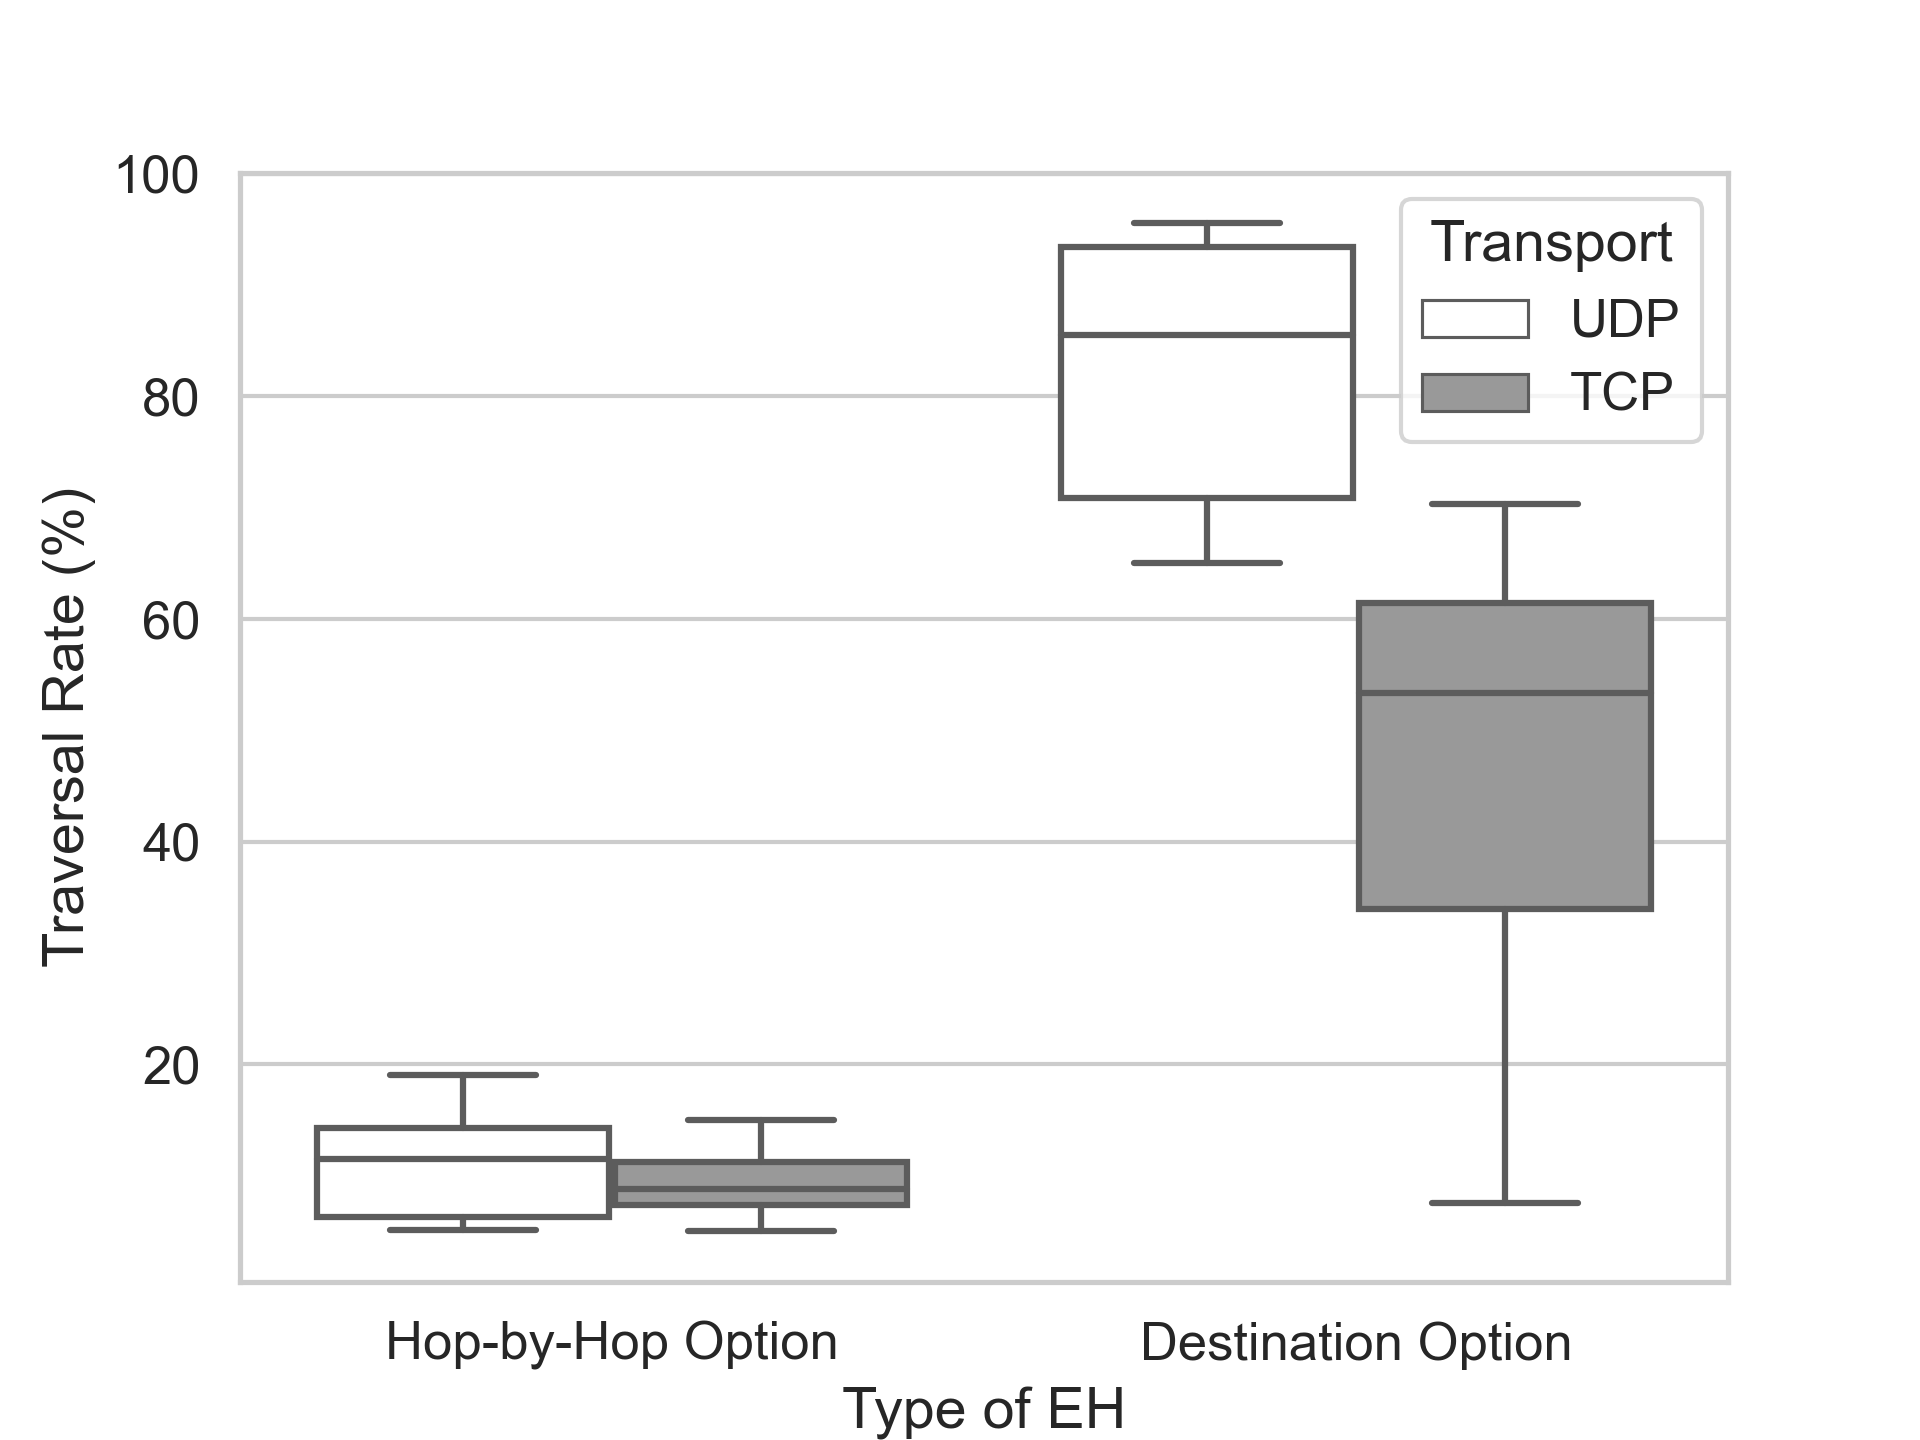
\includegraphics[width=0.5\textwidth]{all_traversal.png}
  \caption{Traversal of HBH and DST from an Atlas vantage points to target servers located in 7 different countries (dataset R1). }
  \label{fig:countrybox}
\end{figure}

\begin{figure}
\centering
  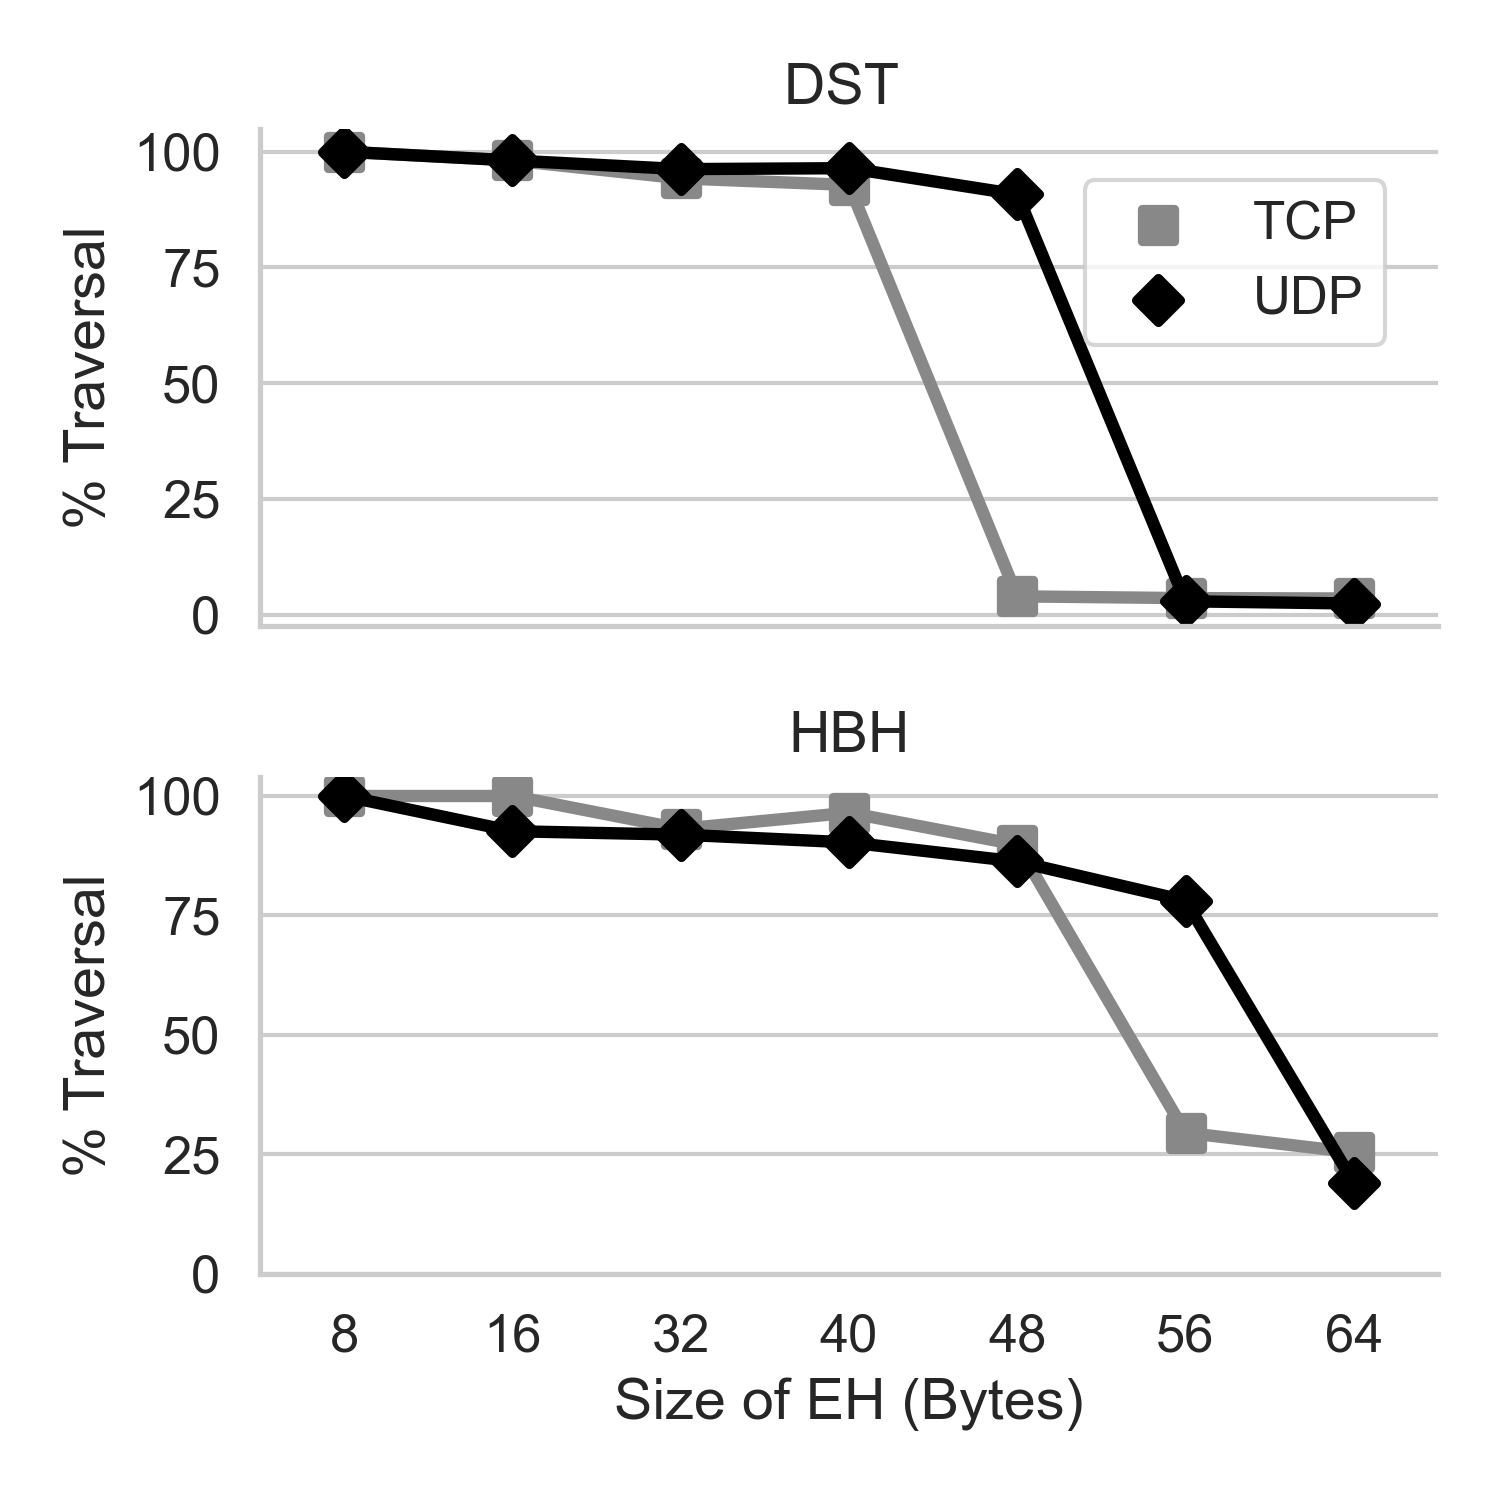
\includegraphics[width=0.45\textwidth]{sizes.png}
  \caption{Traversal percentage forfor packet including HBH and DST EHs from Atlas vantage points to a target server within the JANET network (AS876), per size of EH and split by transport.  Total n=129,585 measurements, with a mean of 4628 measurements ($\sigma$=351) for each combination of transport, size and EH  (dataset R2). This variation in the number of measurements results from availability and connectivity of  probes  with time.}
  \label{fig:sizes}
\end{figure}

\subsection{Pathologies}
    \label{subsec: pathologies}

The results show a very low EH traversal when using TCP towards the Kazakhstan and Zambian target networks. Both have only one BGP peer, and for both, we find that the majority (over 50\%) of TCP packets see their last reply from a router in the destination's upstream AS. In both cases, plotting the path traversal to the AS upstream of the destination AS reveals similar results to targets in other tested countries. This is shown in Figure~\ref{fig:traversal_pathologies}.

\begin{figure}
\centering
  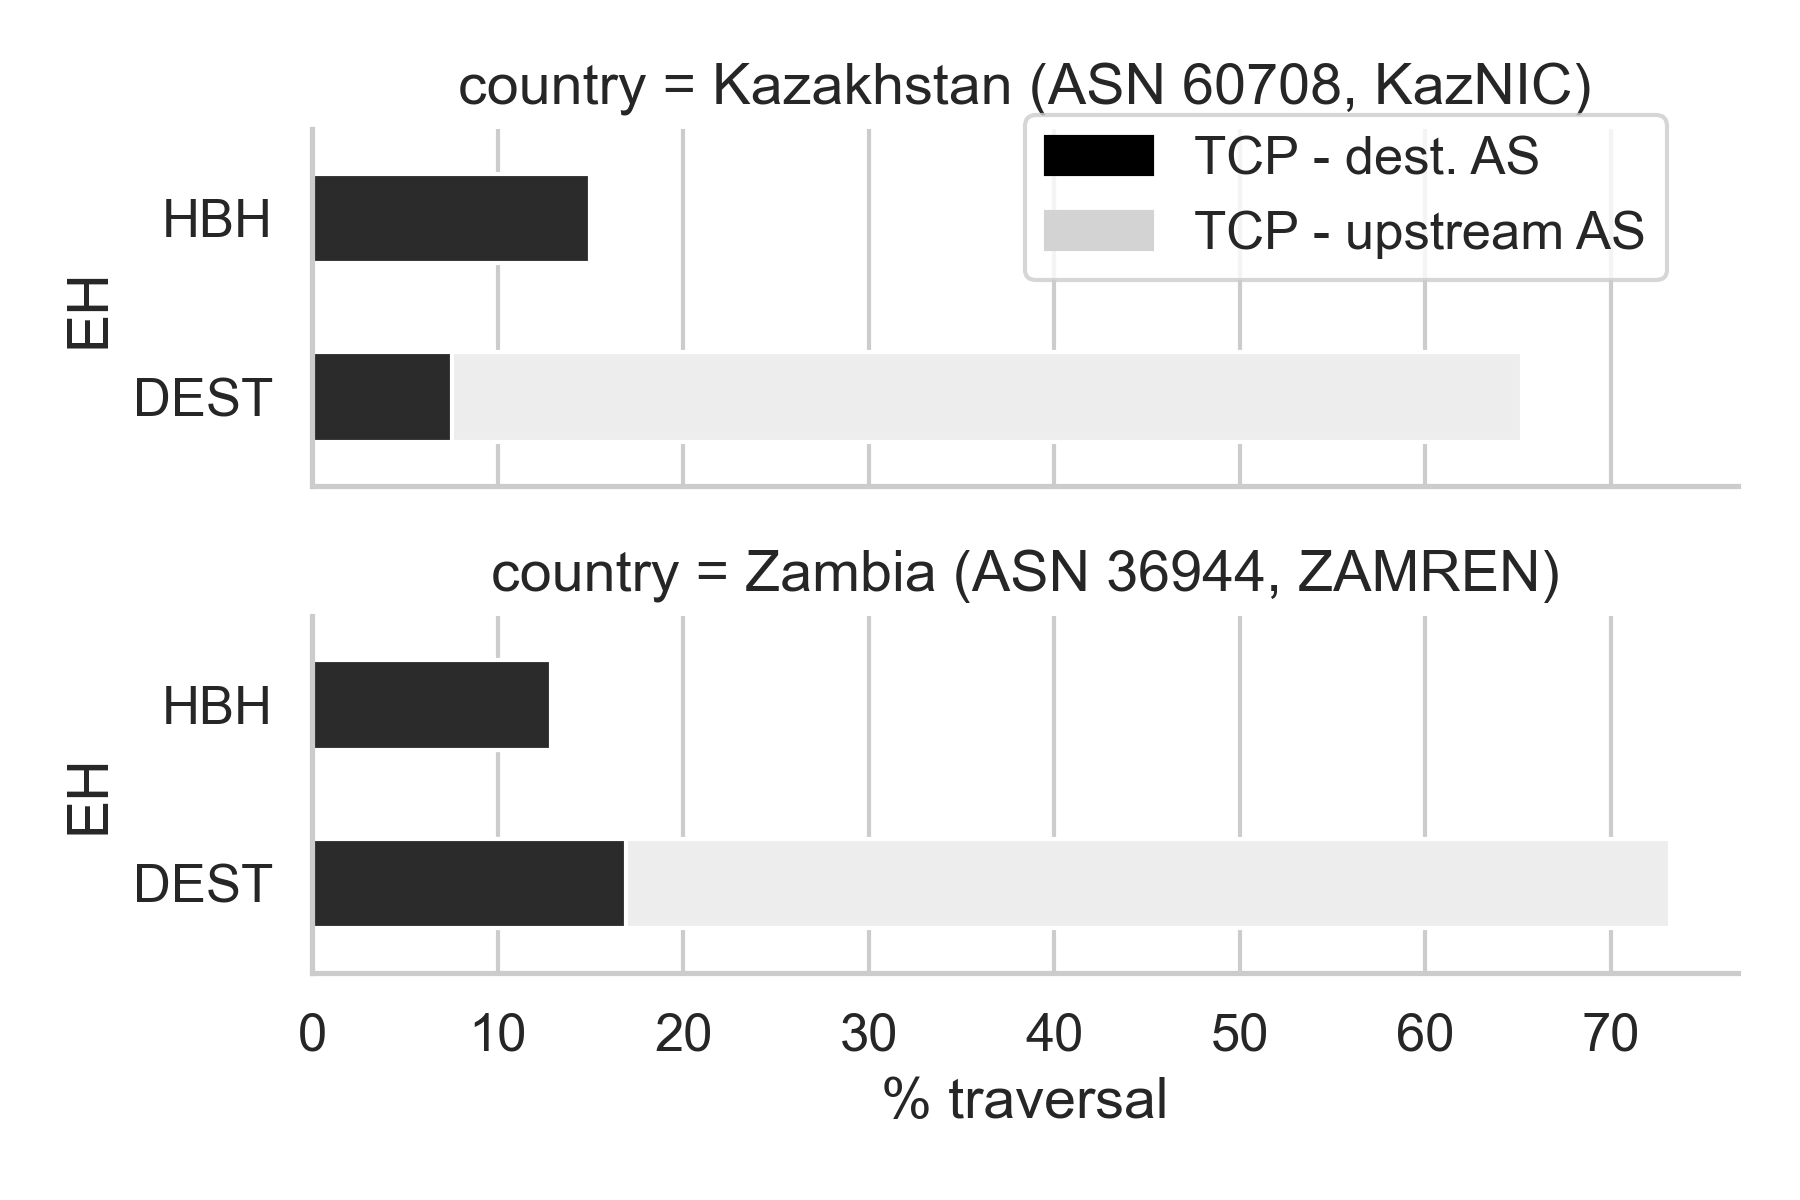
\includegraphics[width=0.5\textwidth]{traversal-pathologies.png}
  \caption{Traversal from Atlas vantage points to both destination and upstream AS for targets in Kazakhstan (n=5075) and Zambia (n=4462). The figure shows the traversal percentage of TCP packets using both types of tested EH.}
  \label{fig:traversal_pathologies}
\end{figure}

Operator mis-configuration can influence traversal: The only BGP peer for the Kazakhstan network is Hurricane Electric (AS6939) and use a  brokering service where the IPv6 peering is tunneled over an existing IPv4 connection to an endpoint located in Dusseldorf. Upon closer inspection, we find that the 7\% of paths where packets traverse to the destination network originate (with 3 exceptions) in ASes located Australia/New Zealand. The 50\% dropped packets that originate in other geographical areas are filtered at the tunnel endpoint. We therefore assume misconfiguration or a policy within the HE transit network routers results in this pathology. 
%They can also come from comcast but somehow they bypass HE?!?!?!?!


The only BGP peer of the target network in Zambia is Ubuntunet Alliance For Research and Education Networking (AS36944). Over 50\% of packets are dropped at the last hop seen in this AS. There is no common origin for the results wherepackets do
traverse, therefore we attribute drops are a result of policy. 

\subsection{Path traversal analysis}

Tables~\ref{tbl:uk_as1} and \ref{tbl:uk_as2} present the percentage traversal at each AS on the path to the UK destination for packets including an 8B EH. We observe the majority of drops occur within the first AS on the path (the vantage point AS) - between 68\% HBH (UDP) and 74\% (TCP) packets and 5\% (UDP) to 25\% (TCP) of DST packets. A difference due to the transport is still observed when the results are split per AS. 

We note packet drops within the source AS are common to all Atlas measurements regardless of destination. Packets including DST using UDP experience a drop rate less than 1\%, as they traverse further  ASes, suggesting that they traverse the Internet core.

We further investigate where packets  including an EH are discarded within the source AS, and find the majority of drops happen at the very first router on the path (i.e. the vantage point's local router).
Figure~\ref{fig:empty_paths} shows the percentages of paths where packets are dropped at the first router - i.e. paths where no traceroute responses are received for test packets, but where responses are received for control packets. Packets that include a HBH are dropped at the local router on more than 50\% of paths. This varies little with the choice of transport (54\% for UDP and 56\% for TCP, for an 8B EH). In contrast, only between 2 and 15\% of paths drop packets that include a DST, and this rate depends on the transport: (2.5\% for UDP and 10\% TCP for an 8B EH). The percentage drop increases with size regardless of which EH was included.


The local routers for this set of vantage points are a diverse mixture of edge routers connecting enterprise LANs, mobile and broadband networks. They perform a variety of functions, including access control, and authentication that usually require access to transport header information. 



A common modification made by edge routers is clamping of the Maximum Segment Size (MSS) option in the TCP header. This is done to avoid problems which otherwise arise from Path MTU discovery. 

xx Below para: isolate I understand, but method not explained xx
xx MSS option or MSS Option XX

There is no way to determine whether a drop is a result of a configured policy, a bug, or a lack of support. 
However, it is possible to identify the paths that insert TCP Options such as the MSS OIption by using a traffic capture tool to collect and examine the Atlas measurement packets as they arrive at the destination server during the baseline measurement. By default, the packets sent from Atlas probes do not include a TCP MSS Option - and therefore if in our examination we find the TCP Option is present at the destination, this means a device on that path has inserted this.

We identify 853 paths where an on-path device has inserted a TCP MSS Option in our baseline measurements to the UK destination. We then look at EH traversal within this subset of paths to determine whether this characteristic makes a difference for overall traversal, on the basis that at least one on-path device will have needed to parse the entire IPv6 Header, including any EHs, to perform this function.
We find a traversal of only 2.6\% for HBH and 48.1\% for DST for this subset of paths, indicating dropping is more prevalent where an on-path device modifies the TCP MSS option.

xx Need to explain what we think this means XXX

\begin{figure}
\centering
  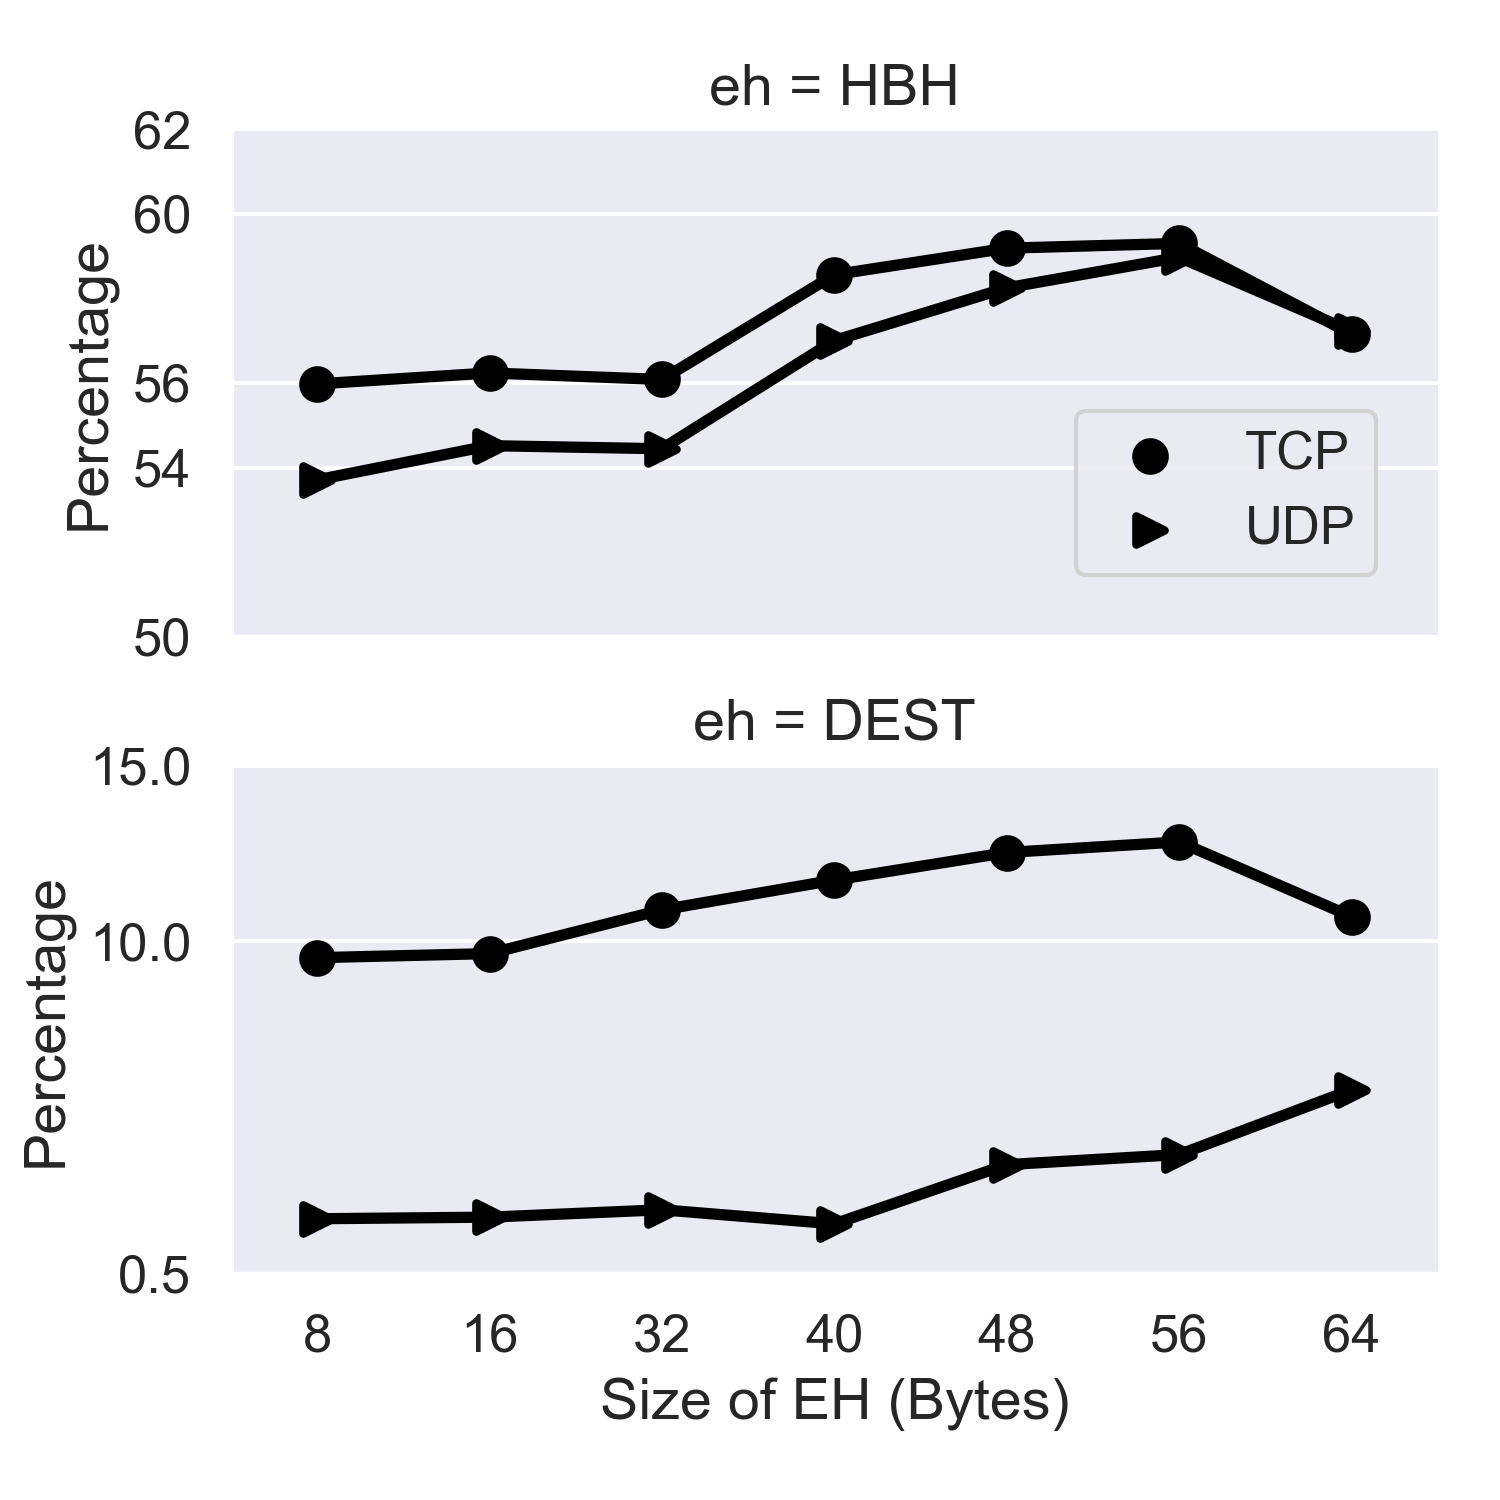
\includegraphics[width=0.5\textwidth]{empty_paths.png}
  \caption{Percentage of paths where packets are dropped at the first router, per EH, transport protocol and size.}
  \label{fig:empty_paths}
\end{figure}


\begin{table}
\centering
\caption{Per-AS drop attribution for 8B DST packets sent from n=4970 Atlas vantage points to a target destination in AS786. The local AS is responsible for the majority (5\% for UDP and 25\% for TCP) of the drops.}
 \label{tbl:uk_as1}

\begin{tabular}{l|l|l|l}
                                   & 1st AS & AS1\textgreater AS2 & $inf $     \\ \hline 

{Dest UDP 8B} & 95.3\% & 93\%                 & 91.5\% \\ \hline

{Dest TCP 8B} & 74.7\% & 70\%                 & 68.5\%
\end{tabular}
\bigskip
\caption{Per-AS drop attribution for 8B HBH packets sent from n=4970  Atlas vantage points to a target destination in AS786. The local AS is responsible for the majority (68\% for UDP and 74\% for TCP) of the drops.}
\begin{tabular}{p{0.07\textwidth}|l|l|l|l|l}

              & 1st AS & AS1\textgreater{}AS2 & 2nd AS & AS2\textgreater{}AS3 & $inf$     \\ \hline
HBH UDP 8B & 31.4\% & 20.1\%               & 15\%   & 12.2\%               & 11.4\% \\ \hline
HBH TCP 8B & 26.9\% & 16.3\%               & 13.9\% & 9.7\%                & 8.6\%  \\ 
\end{tabular}
 \label{tbl:uk_as2}
\end{table}


\subsection{Internet path analysis}

Load balancing routers are another type of on-path device that can be configured to read  the upper layer headers of a packet. We perform Paris Traceroute measurements todetermine whether this function is impacted by a packet that includes an EH. This tool aims to detect the presence of load balancing on a given path~\cite{augustin2006avoiding}, by performing multiple traceroute measurements varying several header fields (a `Paris variation'); on-path devices may use several fields for load-balancing. To identify the packets sent for a specific measurement, Paris Traceroute idebntifies each variation basedon either the TCPsequence number field or the UDP checksum field

Six sets of measurements were run from  vantage points to the Zambian destination, with each measurement set using 16 Paris variations. We select the vantage points and destination based on previous measurements so as to only measure complete paths, where traversal always succeeds, 766 paths in total. The Paris Traceroute version used by Atlas varies the IPv6 Flow Label and transport port number deterministically between individual Paris measurements. Each group of 16 Paris measurements forms a measurement set. The same 16 combinations of IPv6 Flow Label and port number are used for subsequent measurement sets.

\begin{figure}
\centering
  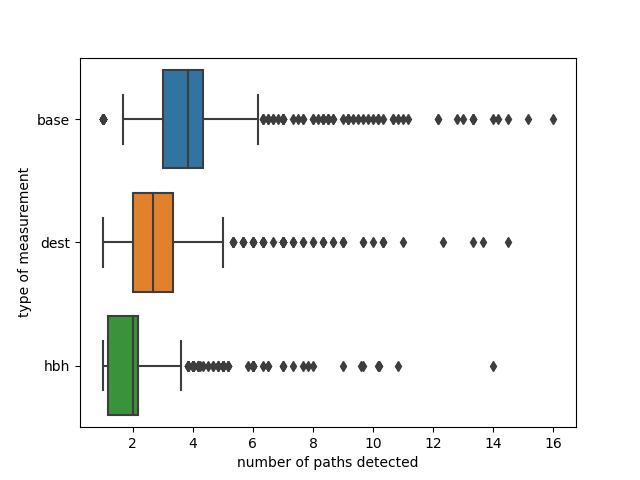
\includegraphics[width=0.5\textwidth]{boxplot-paths-detected.png}
  \caption{Number of paths detected by Paris Traceroute in 866 source-destination pairs, averaged over 5 measurement runs, with each run using the same 16 Paris variations. The baseline measurement using vanilla packets is compared against DST and HBH measurements (dataset R3).}
  \label{fig:paths-detected}
\end{figure}

Figure~\ref{fig:paths-detected} compares how many paths are discovered using Paris Traceroute when using vanilla IPv6 packets versus packets that include an 8B DST or HBH EH.
A total of 16 Paris variations discovered on average 4 paths~\cite{augustin2006avoiding}. We reproduce this in our baseline results, finding a median of 4.1 paths. However, the medians for measurements where packets carried an 8B DST or HBH EH are 2.96 and 2.1 respectively (Figure~\ref{fig:paths-detected}).

XXX above para does not have an outcome sentence at the end! xxx

For 518 (60\%) of source-destination pairs, measurements performed with DST EHs detect the same (+-1 path) number of paths as the baseline. For 328 (38\%) pairs, the measurements detect fewer (by 1 path or more) number of paths than the baseline. On the other hand, measurements using HBH EHs detect the same (+-1 path) number of paths as the baseline for only 115 (13.4\%) source-destination pairs. Much more commonly, fewer paths are detected when this type of EH is used compared to the baseline. This happens on 604 paths (69.7\%). This pathology could happen, for example, if ECMP-enabled routers use a byte offset for their hash calculations. Overall, this means that packets with an HBH EH are less likely to take the same Internet path as a vanilla packet.
XX does not say why this matters XX

For some source-destination pairs, the EH Paris measurements detect at least 1 more path than the vanilla measurements. These cases are rare - around 1\% (8 paths for DST and 10 for HBH), but can however reveal interesting pathologies.
For example, for one pair the baseline measurement detects 4 paths, the DST measurement detects 2 paths, while the HBH measurement detects 14(!) different paths. Upon closer inspection we find a single router that enumerates 14 interfaces, only in the presence of packets containing HBH EHs.
XXX we need a half sentence to conclude whether this sort of problem impacts usage - likely not in this case?

%For 12 source-destination pairs in the dataset, not enough data was gathered using Destination Option EHs to complete a measurement run. Not enough data was gathered for 137 (15.8\%) pairs.
This set of measurements indicates that not all load balancer implementations are well suited for packets carrying the HBH or DST EH.


\section{Pathspider results} 
\label{sec:pathspider-results}

This section presents results obtained with PATHspider~\cite{learmonth2016pathspider}. In contrast to the Atlas measurements, these experiments use a limited number of vantage points and target a large number of destinations. Where the destination is an authoritative NS, PATHSpider first performs a control measurement by sending a DNS query to the server using IPv6 packets not including an EH.
PATHSpider performs an end-to-end test, which measures server support in the destination. Although this requires test packets to traverse the path to the destination, this is not a path traversal measurement.

The same measurement is then repeated using an 8 Byte PadN DST or HBH, and in each case the test is considered successful if the server replies to the DNS query. Where the destination is a web server, the test can only be done over TCP by sending a TCP SYN, and is considered successful if the server replies with a TCP SYN-ACK.
This section reports on the end-to-end support, or the percentage of paths where test packets were observed to receive a response from the destination server.

\begin{table} 
\begin{tabular}{c|cc|cc}
\multicolumn{1}{l|}{} & \multicolumn{2}{c|}{DST Support} & \multicolumn{2}{c}{HBH Support} \\ \cline{2-5} 
\multicolumn{1}{l|}{} & \multicolumn{1}{c|}{TCP}       & UDP      & \multicolumn{1}{c|}{TCP}     & UDP     \\ \hline
UK                    & \multicolumn{1}{c|}{69.1}      & 69.3    & \multicolumn{1}{c|}{12.5}    & 15.8  \\ \hline
Canada                & \multicolumn{1}{c|}{76.3}      & 76     & \multicolumn{1}{c|}{23.3}    & 24.2  \\ \hline
Australia             & \multicolumn{1}{c|}{72.5}        & 72.2      & \multicolumn{1}{c|}{17.7}    & 17.5  \\ \hline
Singapore             & \multicolumn{1}{c|}{72.8}      & 72.7    & \multicolumn{1}{c|}{17.4}    & 17.4   \\ \hline
Poland                & \multicolumn{1}{c|}{76.5}      & 76.8   & \multicolumn{1}{c|}{24.4}    & 24.7   
\end{tabular}
\label{tbl:e2e_traversal}
\caption{End-to-end support for an 8B Pad N option for both Dest and HBH EHs, from vantage points in 5 countries to n=18002 unique authoritative NSes in the Cisco Umbrella Top 1M, in 2787 different known ASes. All measurements performed in February 2023, part of dataset P1. }
\end{table}

\begin{table} 
\begin{tabular}{c|c|c|c}
           & \% of dataset & Supports DST & Supports HBH \\
\hline
Cloudflare & 18                      & Yes                & No                 \\
\hline
Amazon     & 11                     & No                 & No                 \\
\hline
Hetzner    & 3                     & Yes                & No                 \\
\hline
Gandi      & 4                     & No                 & No                 \\
\hline
Ionos      & 3                    & Yes                & No                
\end{tabular}
\label{tbl:provider_support}
\caption{End-server support for the DST and HBH for major DNS server providers, n=99,987 paths, based on measurements from December 2022. Google does not support either option, and is not listed in the table as it only had 30 destinations in the dataset.
}
\end{table}

\subsection{End-to-end support}
\label{subsec:e2esupport}

Table~\ref{tbl:e2e_traversal} presents the end-to-end support for the authoritative NSes for the current Cisco Umbrella top 1M Domains list (Feb 2023).
% ANA TODO - double check results^

Similar to the access network results previously presented, support varies between the DST and HBH EHs: 69 to 80\% of the tested servers replied to packets using DST, and up to 24.2\% do so for HBH. Traversal does not vary with transport in the same way seen for the access network results presented in the previous section. We attribute this to the lack of edge router devices normally present in access networks. Only one measurement, from the Singapore vantage point, sees a 5\% difference based on transport in favour of TCP for both EHs tested.
Finally, the table shows variations in support based on vantage point - support varies between 12 to 24.7\% for HBH, indicating fewer packets dropped in transit networks in the latter case.

However, around one third of destinations in the DNS dataset featured in Table~\ref{tbl:e2e_traversal} are hosted by a few major hosting companies (Cloudflare, Amazon, Gandi etc.) which employ network policies to filter packets with some EHs in their network. End-server support for major DNS server providers are presented in Table~\ref{tbl:provider_support}. In Early December 2022, Cloudflare servers started responding to DNS queries sent with packets including DST, this results in a jump from 57\% to over 70\% for the dataset. If all major providers would enable support, this would bring the success of the E2E test to over 90\% for DST and 60\% for HBH for this dataset.

We tested end-to-end support for webservers in the Cisco Umbrella top 1M Domains list (232350 unique IP addresses, Feb 2023) from the same destinations. This list of webservers is much more dominated by a few major hosting companies: around 52\% of destinations are hosted by Amazon Inc (AS16509); 23\% are hosted by Cloudflare (AS13335), and around 2.5\% each are hosted by Akamai Technologies and Google. We break down supported EHs for each in Table~\ref{tbl:web_provider_support}. We find more than two-thrids of Amazon-hosted webservers respond to connections over packets with DST, in contrast to Amazon-hosted DNS servers, where none do. 

Overall, we find end-to-end support for all tested webserver addresses to be between 72 and 78\% for DST packets and between 2-3\% for HBH.


\begin{table} 
\begin{tabular}{c|c|c|c}
           & \% of dataset & Supports DST & Supports HBH \\
\hline
Amazon & 52                      & Yes                & No                 \\
\hline
Cloudflare     & 23                     & Yes                 & No                 \\
\hline
Akamai    & 2.7                     & Yes                & No                 \\
\hline
Google      & 2.3                     & No                 & No                 \\
\
\end{tabular}
\label{tbl:web_provider_support}
\caption{End-server support for the DST and HBH for major webserver providers, n=99,987 paths, based on measurements from December 2022. Google does not support either option, and is not listed in the table because it only had 30 destinations in the dataset.
}
\end{table}


\subsubsection{Option Type support}

We repeated the DNS server experiment described above from one vantage point, varying the Option Type and Option Lnegth fields. 
Table~\ref{tbl:option_type_support} shows the support for different Option Types within the authoritative NSes for the current Cisco Top 1 Million Domains. We test a well-known option, PadN~\cite{rfc2460}, against a recently-standardized one - Minimum Path MTU HBH~\cite{rfc9268}. We also test two experimental options, 30 and 254~\cite{RFC4727}. The latter was chosen to test the traversal when the Option Type has its two most significant bits set.
We find that the Option Type does not affect traversal where the two most significant bits of the field are not set - with the same traversal percentage for PadN,minPMTU Discovery and Experimental Option 30. Where the highest order bits are set, traversal is expected to be 0 - however, we still receive responses on 0.4\% of paths, indicating all devices on that path have ignored these bits.

The same applies for an incorrectly set Option Length field. Any device parsing the EH field should validate the Option Length set for each option, traversal is expected to be 0; however we still find a small number of paths (0.5\%, or around 80 paths) where all devices on the path ignore this field.

\begin{table}
\begin{tabular}{l|l|l}
Test                      & DST EH & HBH EH \\
\hline
Pad N option (1)          & 69.3           & 15.1          \\
PMTU Discovery (48)       & 69.5           & 15.8          \\
Experimental Option (254) & 0.4            & 0             \\
Experimental Option (30)  & 69.4           & 15.1          \\
Incorrect Option Length   & 0.5            & 0.05            
\end{tabular}
\label{tbl:option_type_support}
\caption{End-to-end support for different Option Types in the authoritative NSes for the Cisco Top 1 Million Domains, n=19052 unique IPv6 targets. The transport used was UDP (dataset P2).}
\end{table}

\subsubsection{ICMP Unreachable Messages}

When a packet with a HBH Opt is sent, but does not receive a reply (i.e. the packet is dropped by the path),  ICMP unreachable messages are seen on 0.2\% of the tested NS paths. For DST packets, ICMP unreachable messages are seen on between 0.3 and 8.8\% of paths, depending on vantage point.
This suggests that ICMP messages cannot be used to ascertain whether a packet carrying options was dropped in transit.
Upon closer inspection, we also find that for all destinations, ICMP unreachable messages can be received even when the test succeeds on up to 2\% of paths. These are exclusively received from routers in destination ASes and indicate misconfiguration.


\subsubsection{ICMP Parameter Problem Messages}

When a packet carries a Dest or HBH which has its two MSBs set, routers that do not understand this option should discard packets with this option and return an ICMP Type 4 Parameter Problem message back to the sender. To examine whether this is prevalent in the Internet, we repeat the DNS server experiments using packets using experimental Option Type 254. This option has its two MSBs set and is unlikely to be understood by any routers, and therefore we expect any sent packets to be dropped.

Behaviours for DST and HBH respectively are described in Table~\ref{tbl:icmp_support_dst}.

In the case of DST, for all vantage points tested, only the gateway router local to the vantage point returns ICMP Type 4 Parameter Problem messages for the packets sent, as expected; the percentage of destinations for which the ICMP messages are received varies between 50-100\%. Because the local router always generates these messages, we attribute this variation to ICMP rate-limiting. 

In the case of Hop-by-hop options, we find that while the local gateways in all vantage points forward the packets,  ICMP Type 4 Parameter Problem messages are received from intermediary routers on the path or in the destination AS. The response rate varies between 52 and 73\%. 

For both EHs tested, due to ICMP rate-limiting and filtering, this mechanism is not found to be a reliable indicator on whether or not a packet with an unknown option with its two MSBs set is dropped. We also find that on many paths, packets with Hop-by-Hop Options are forwarded nevertheless.

In addition, for DST packets, on between 0.2 and 0.5\% of paths, we also find that despite sending this message, the local router also forwards the packets to the destination and a response is still obtained by the server (the end-to-end test succeeds), which could indicate a router implementation issue.

\begin{table}
\begin{tabular}{p{0.12\textwidth}|p{0.04\textwidth}|p{0.03\textwidth}|p{0.03\textwidth}|p{0.03\textwidth}|p{0.03\textwidth}|p{0.025\textwidth}}

\centering

                                           &             & UK        & Can       & Aus    & Sgp          & Pol     \\
                                           \hline

{\% ICMP received in vantage AS}        & {HBH DEST} & {0 100}  & {0 51.6}    & {0 51.9}    & {0 51.9}    & {0 51.5}  \\
\hline
{\% ICMP received elsewhere on path}          & {HBH DEST} & {72.8 0} & {52.5 0}    & {68.2 0}    & {69.2 0}    & {73  0}    \\
\hline

{\% ICMP received, packet forwarded}          & {HBH DEST} & {0 0.52} & {0 0.48}    & {0 0.46}    & {0 0.24}    & {0 0.46}  \\
\hline

{\% ICMP message not received} & {HBH DEST} & {27.2 0} & {47.5 48.4} & {31.8 48.1} & {30.8 48.1} & {27 48.5} 
\end{tabular}
\caption{Different behaviours for ICMP rate-limiting.}
\label{tbl:icmp_support_dst}
\end{table}

\subsubsection{Longitudinal support}

Table~\ref{tbl:longitudinal_support} presents measurements across the same set of domains over the course of 3 years. Each domain was resolved prior to the measurement, resulting in a variation of the total unique IP addresses tested, presented in the last table row. The results show a trend towards lower support for HBH, with DST support remaining constant over time, until December 2022 when Cloudflare enabled support as described in Subsection~\ref{subsec:e2esupport}.

% Ana: verify total number of paths.
\begin{table}
\begin{tabular}{l|l|l|l|l}
                    & Jan 2020 & Jul 2020 & July 2022 & Dec 2022 \\
\hline
DST & 59.9\%   & 54.3\%   & 57.4\%    & 71.7\%   \\
HBH  & 25.7\%   & 23.8\%   & 16.4\%    & 11.9\%   \\
\hline
Unique IP addresses & 18296    & 19690    & 19553     & 20050   
\end{tabular}
\label{tbl:longitudinal_support}
\caption{End-to-end support for an 8B Pad N option for both Dest and HBH EHs, from one vantage point to the authoritative NSes for the same set of 1M domains, between Jan 2020 and Dec 2022 (dataset P1). The transport used was UDP.}
\end{table}

\subsection{AS analysis }



Table~\ref{tbl:as_pathspider} presents ASes targeted by Pathspider (2868 in total) alongside evidence that they support either the DST or HBH EH.
If at least one reply is seen from that AS to one of our test packets from any of the locations tested, we consider that AS supports the traversal of packets using the tested EH type. Thus, at least 92.4\% of destination ASes allow traversal of packets including an 8B DST EH, and more than half, 53.8\%, allow an 8B HBH EH. The percentage reducess for multiple paths towards that AS, revealing that many packets including an EH are dropped in an AS  that is different from the destination AS. For DST, 3.4\% fewer ASes permit DST traversal on more than half the paths, whereas for HBH, the difference is 16.6\%.
When only considering the subset of ASes (1606) tested over 10 or more paths, the results vary little: at least 93.2\% of destination ASes allow traversal of packets including an 8B DST EH, and more than half, 55.9\%, allow an 8B HBH EH.

    \begin{table}
\begin{tabular}{p{0.195\textwidth}|p{0.11\textwidth}p{0.118\textwidth}}
                                          & Paths per AS$>$=1 & Paths per AS$>$=10 \\ \cline{1-3} 
Total number of ASes                      & 2787                                            & 1606                                            \\ \hline
AS does not support DST               & 212 (7.6\%)                                     & 110 (6.8\%)                                     \\
AS supports DST on 1 or more paths   & 2575 (92.4\%)                                   & 1496 (93.2\%)                                   \\
AS supports DST on 50\% paths or more & 2476  (88.8\%)                                  & 1437 (89.4\%)                                   \\ \hline
AS does not support HBH               & 1287 (46.2\%)                                   & 709 (44.1\%)                                    \\
AS supports HBH on more than 1 path   & 1500 (53.8\%)                                   & 897 (55.9\%)                                    \\
AS supports HBH on 50\% paths or more & 1037 (37.2\%)                                   & 580 (36.1\%)                                   
\end{tabular}
\label{tbl:as_pathspider}
\caption{Number of ASes where DNS servers can be reached via packets carrying either Dest or HBH. The first column considers all destination ASes in the dataset, while the second only looks at ASes that host 10 destination addresses or more. Based on measurements from December 2022 (dataset P1).}
\end{table}

\section{Discussion} 
\label{sec:discussion}

Since its standardisation, the IPv6 protocol has
seen widespread adoption~\cite{v6adoption_ton} and the hardware and software that
support it have matured: packet parsing capacity in routers is increasing and
router architectures have evolved~\cite{metamorphosis, p4}, including solutions based on re-configurable
logic circuits that can enable new functions to be introduced~\cite{cisco-silicon-one}.

We find that packets including the DST EH traverse on up to 96\% percent of Internet paths and that over 92\% of server edge ASes allow support.
Packets with HBH are still currently dropped in transit networks (validated in Table~\ref{tbl:as_pathspider}) and in access networks in Figure~\ref{fig:countrybox}, although when measuring server edge targets we find that up to 50\% of ASes allow support. Mis-configuration or other network policies can result in pathologies within transit networks, shown in Subsection~\ref{subsec: pathologies}. We also find that traversal for both DST and HBH drops significantly on paths containing edge-network devices that insert a TCP transport option.


Updates have also been made to the IPv6 standard based on
operational experience~\cite{RFC5722}~\cite{RFC6946}~\cite{RFC6564}~\cite{RFC8200}. EH processing has become a recent focus in the standards community, that seeks to motivate a change in both network operator policies and the implementation of more robust router architectures that facilitate EH processing~\cite{ietf-6man-HBH-processing-06, ietf-v6ops-HBH-03, ietf-6man-eh-limits-02}. 


%Question 1: do extension header actually traverse common Internet paths? Is there a longitudinal trend making this more easy or harder?


Server-side, testing for the same set of NSes between 2019 and 2022 reveals the support for 8B PadN HBH decreases over time when considering individual destinations (Table~\ref{tbl:longitudinal_support}) as more NS servers become centralised under only a few ASes that do not support HBH.  However, an analysis of AS results reveals more than half of the tested ASes allow packets carrying a HBH EH and more than 90\% allow packets carrying a DST EH. The AS analysis confirms that transit networks can present an obstacle to deployment of the HBH EH.
 
RFC 7872~\cite{RFC7872} describes the traversal to the authoritative NSes for the Alexa Top 1M domains in 2014. This observes packets carrying an 8B PadN DST traverse paths to  78.6\% of destinations and packets carrying an 8B PadN HBH traverse to 45.9\% of destinations. These results were measured from a single vantage point and are not grouped per AS, and so can be compared with results in Table~\ref{tbl:longitudinal_support}, which indicates a 5-9\% decrease in support for DST and a 25-30\% decrease in support for HBH, although we note this could reflect changes within the top 1M domain list itself between 2014 and 2023.
This AS analysis reveals that packets with Options traverse to up to 90\% and over 50\% of ASes respectively, we can infer the decrease is due to drops within the destination AS.

% should we add a para here (GF: Yes, but: NOt here, but in discussion - since it isn't our thesis of thus paper) about whether dst opts are even useful across the internet? 
% makes sense to use them within domains, where encryption is not needed, but perhaps in an 'untrusted' domain quic etc is better

Since the HBH (and first DO) comes before the routing header, this has to be processed or skipped for any router that acts as an SRv6 intermediate node to allow it to update the destination address using the routing EH.

XXX
Refer to SRV6
- probably should use this to link to SRv6 to an example use  case such as Service Function Chaining and Network Function Virtualization.
https://ieeexplore.ieee.org/document/9253580

XXX

%Question 6: what is the opportunity for destination options? Is it a good trade-off to have a network layer? That is consistent transport header or is it wiser to put the transport header information within the transport and therefore allow it to be encrypted such as quic transport parameter - so what is the real advantage of destination options?

%Question 2: is there a limit to extension headers that prevents them from traversing certain Internet paths such as limiting length of the EH chain or a specific EH length? Would ? Is it different between HBH and DO?

EH chains of up to 40B in size sent over UDP have the highest chance of traversing access network paths, shown in Figure~\ref{fig:sizes}.
For a total IPv6 header and transport chain of under 104B. This suggests that when using EHs, keeping packet sizes under this limit may help in ensuring consistent deployment.

%Question 4: is there a possibility to deploy a different new option...is this sensitive to the format of the option or the presence of a new defined option? This is a part whether a specific option causes the traverse ability to change, or whether an illegal format option changes the traversability of the packet.

We also find that traversal does not depend on the type of Option included (see Table~\ref{tbl:option_type_support}). This is important because it permits a new DST or HBH Option to be defined and then used on a path that supports EH processing (e.g., the Minimum PMTU  Option~\cite{rfc9268}), because their traversal is not expected to require deployed infrastructure to be updated. Updates would only be needed to add new functionality in routers where the Option needs to change the processing.

%Question 3a: When options extension headers do traverse, do they traverse consistently for the same pair of endpoints?
%Quetsion 3b: Does the flow label help to ensure a consistent set of network devices on a path? -- If not, then we ought to suggest the step towards evolution would be to add a PAD option to all packets that would not otherwise have an EH?
%Question 3c: Is there a trend to set meaningful entropy in the flow label against the original place where many endpoints sent a zero value flow label?
%Question 3d: Is the flow label invariant .... is the FL the same at src as at the dst ...  (i.e. do devcies on-path rewrite) is that something RIPE could easily answer. - If they reset to zero then they are evil!
%Here we should not forget the proposals to add flow metadata as a hop by hop extension to let network devices know helpful information to consider how to fold the packets in a flow.

%Question 5: If we find HBH don’t work everywhere then ….What is the opportunity for using a hop by hop extension header on some of the packets belonging to a flow? does this result in new forwarding pathologies? That is where the packets that include EHs take a different set of devices to the packets with no extension headers, and if so do they take a different network or do they simply follow a different path through the same operator network? Does this result in inconsistent loss? Is the option useful ?


Results presented in Figure~\ref{fig:paths-detected} show that including an EH in a packet may change its forwarding path. We note that both the Flow Label and the source port of packets were varied to detect paths between the same pair of endpoints. EHs sit between the IPv6 header (which contains the flow label) and the transport header (which contains the source port), suggesting some load-balancing networking equipment use a byte offset expected to contain the source port, and that the flow label is not used in all cases. Overall, this means traffic flows that mix packets including these EHs and packets without must take care as these may not travel on the same Internet path.

XX Is there ANYTHING we can cite on Flow Label trends? Is this helpful: https://ieeexplore.ieee.org/document/7014534  XXX

Our results also show that most routers are configured to discard packets and send ICMP messages as specified by~\cite{RFC4443} when encountering an option that cannot be processed. However, we still find instances where a router sends this message in response to a DST EH that has both most significant bits set, but packets are forwarded nevertheless; more commonly, packets that include a HBH EH with both most significant bits set are forwarded without sending an ICMP message. Overall, ICMP is not found to be a reliable mechanism for indicating whether or not packets including an EH is forwarded. 

While access control lists are necessary in some networks today to protect devices where EH processing leads to DoS vulnerabilities or undesirable side-effects, in cases where this is not needed, such a policy is an unnecessary barrier that results in ossification that obstructs new uses of EHs.


\section{Conclusion}
\label{sec:conclusion}


IPv6 is actively being extended within isolated domains. This is low risk because domain owners control all their hardware and can deploy the options specified in RFCxxx and RFCyyy

Across the Internet, we find traversal of HBH and DST is variable depending on EH, size, transport and type of network. We find these EHs can impact the function of load balancing routers or of devices that modify transport headers, and that deploying them in the Internet needs to take into account the type of network these will travel over, and carefully consider whether to add them to packets in a stateful flow.


Packets including DST can already traverse many paths both within the core of the Internet, and at the server and network edge. In the case of packets including HBH, 
EH processing has become a recent focus in the standards community, aiming to motivate the implementation of more resilient router architectures that facilitate it~\cite{ietf-6man-HBH-processing-06, ietf-v6ops-HBH-03, ietf-6man-eh-limits-02}. 
It is expected this will help foster the development of new Options and motivate a shift to more permissive network operator policies.




\bibliographystyle{abbrv}
\small
\bibliography{main,rfc}


\end{document}
